\documentclass[9pt,a4paper,DIV=11]{scrartcl}

\usepackage{listings}
\usepackage{color}

\usepackage{graphicx}

\usepackage[ngerman]{babel}

\usepackage{subfigure}

\usepackage{float}

\usepackage{fancyhdr}

%bibtex
\usepackage[square,numbers]{natbib}

\usepackage{dirtree}

\usepackage{gensymb}
\usepackage{textcomp}
\usepackage[tbtags]{amsmath}
\pagestyle{fancy}
%kopf & fußzeile bereinigen
\fancyhf{}
\usepackage[utf8]{inputenc}

\usepackage{hyperref}
\hypersetup
{
colorlinks = false,
linkcolor = black,
hypertexnames = false,
citecolor = green
}

\titlehead
{

\includegraphics[width=0.20\textwidth]{files/hspflogo.pdf}\\

Hochschule Pforzheim\\
Fakultät für Technik
}

\title
{
ROS auf dem KUKA youBot\\
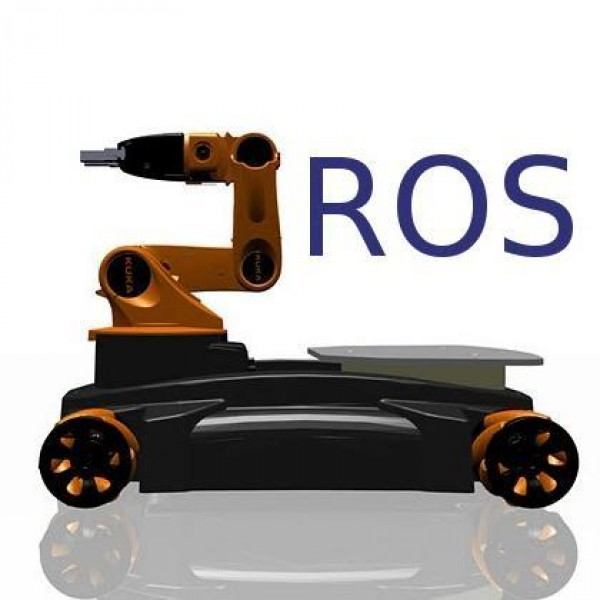
\includegraphics[width=0.20\textwidth]{files/youbot_ros.jpg}
}

\date{\today{}}
	
\author{Jonathan Schwarz - schjon02@hs-pforzheim.de}
\date{\today{}}

\fancyfoot[L]{\textbf{ROS auf dem KUKA youBot} \newline Jonathan Schwarz}
\fancyfoot[R]{Seite \thepage}

\renewcommand{\footrulewidth}{0.5 pt}
\usepackage{lmodern}
\addtokomafont{sectioning}{\rmfamily}
\setlength{\parindent}{0mm}

\definecolor{dkgreen}{rgb}{0,0.6,0}
\definecolor{gray}{rgb}{0.5,0.5,0.5}

\lstset
{ 
  language=C++,                
  basicstyle=\footnotesize,           
  numbers=left,                   
  numberstyle=\tiny\color{black},  
  stepnumber=1,                 
  numbersep=5pt,                 
  backgroundcolor=\color{white},      
  showspaces=false,             
  showstringspaces=false,         
  showtabs=false,                
  frame=single,                   
  rulecolor=\color{black},       
  tabsize=4,                     
  captionpos=b,                   
  breaklines=true,                
  breakatwhitespace=false,       
  title=\lstname,                    
  keywordstyle=\color{blue},          
  commentstyle=\color{dkgreen},       
  stringstyle=\color{blue},      
  escapeinside={\%*}{*)},      
  morekeywords={*,...},            
  deletekeywords={...}             
}


\begin{document}

\renewcommand*\contentsname{Inhalt}
\renewcommand*\listtablename{Tabellen}
\renewcommand*\listfigurename{Abbildungen}

\maketitle
\thispagestyle{empty}
\newpage
\tableofcontents
\newpage
\section{Einführung}
\subsection{Was ist ROS?}
ROS \textit{<<Robot Operating System>>} ist ein Metabetriebssystem für Roboter. Es stellt typische Dienste eines Betriebssystems wie Hardware-Abstraktion, Gerätetreiber, die Implementation von häufig genutzen Funktionalitäten, die Interprozesskommunikation und das Paketmanagment bereit. Das System beseteht aus verteilten Prozessen (Knoten), die lose gekoppelt werden. ROS ist Open Source und hat sich zum Ziel gesetzt, die Wiederverwendung von Code in der Roboterforschung und -entwicklung zu unterstützen. Es existieren bereits Implementierungen des ROS Frameworks in C++, Python und Lisp. Des Weiteren wird der Softwaretest im Software Engineering Prozess durch ein integriertes Testframework und die intergration von Simulatoren erleichtert. Existierende ROS-Pakete stellen bereits Kernfunktionen der Robotik (Navigation, Manipulation, Wahrnehmung, ...) bereit. 
Das Paketmanagment und die bereitgestellte Kommunikation zwischen Knoten im System ermöglicht die einfache, parallele Entwicklung von Softwaremodulen, die gemeinsam einen Roboterapplikation bilden. Dies ermöglicht auch die einfache Integration von Fremdsoftware in das eigene Projekt durch definierte Schnittstellen im System. Es existieren u.a. ROS-Treiber für den Aldeberan NAO und Lego Mindstorm NXT Roboter. Des Weiteren lassen sich durch URDF \textit{<<Unified Robot Description Format>>} selbst gebaute Roboter beschreiben. Dies ermöglicht z.B. die Zusammenarbeit dieser Maschinen.
Als Einarbeitung werden an dieser Stelle die ROS Tutorials \cite{ROSTUT} empfohlen. Für fortgeschrittene Projekte wird \citep{ROSBYEX} als Einführung in bereits implementierte und sehr mächtige ROS-Softwaremodule empfholen. 

\newpage
 
\section{Drahtlose Verbindung}

Um eine barrierefreie Steuerung und Überwachung der mobilen Roboterplattform zu gewährleisten, kann über SSH auf den internen PC des youBot zugegriffen werden. Dazu muss der WLAN Stick mit dem Roboter verbunden sein.
Im Folgenden sind folgende Schritte durch zu führen:

\begin{itemize}
\item[1.] Den internen PC und des steuernden PC im selben Drahtlosnetzwerk verbinden.
\item[2.] \textit{IP} des internen PCs herausfinden. Unix-Kommando: \textbf{\$ ifconfig}
\item[3.] Verbindung über SSH herstellen: \textbf{\$ ssh youbot@\textit{IP}}
\end{itemize}

Nach der Authentifizierung kann jegliche Software auf dem PC ausgeführt werden. Die Drahtlosverbindung erlaubt auch die Steuerung mehrerer Maschinen durch ein ROS-Systems \cite{MULTIROS}.
\section{ROS Wrapper der youBot API}

Die Ansteuerung des youBot Arms und der omnidirektionalen Plattform im ROS Framework erfolgt über das Senden von Nachrichten an ein entprechendes Topic. Abbildung \ref{fig:msg} zeigt die Struktur des ROS Wrappers. Die genutzten Nachrichten sind standard ROS-Nachrichten. Ihr Inhalt kann durch den Befehl \\

\textbf{\$ rosmsg show \textit{Nachricht}.msg} \\

angezeigt werden. Diese Art der Kommunikation wird in Kapitel \ref{sec:src} verdeutlicht.

\begin{figure}[H]
\centering
	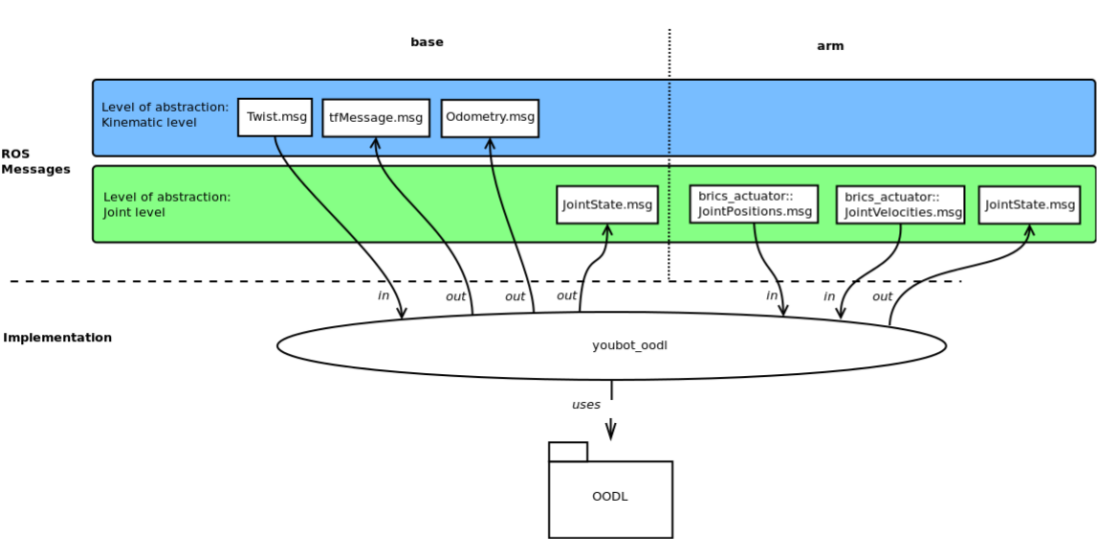
\includegraphics[width=\textwidth]{./files/oodl_ros.jpg}
\label{fig:msg}
\caption{Integration der youBot API ins ROS Framework nach \citep{YBUSER}}
\end{figure}

KUKA stellt bereits einige einfache ROS-Applikationen für den Roboter bereit. In diesen quelloffenen Projekten werden alle Achsen des Roboters angespreochen. Ebenfalls ist eine komplette Beschreiung enthalten, die z.b. zur Simulation und Überwachung mit den Programmen \textit{RViz} und \textit{Gazebo} genutzt werden kann.

\newpage
\section{Microsoft Kinect}
\subsection{Gründe für die Verwendung}
Die Verwendung dieser Tiefenkamera erlaubt das Erzeugen einer dynamischen Karte der Umgebung des Roboters. Dies wird benötigt um fortgeschrittene Konzepte wie SLAM \textit{<<Simultaneous Localization and Mapping>>} zu nutzen. Dies ermöglicht einem Roboter, nicht nur, eine Karte einer unbekannten Umgebung herzustellen, sondern auch die Positionierung in dieser Karte. So kann z.b. Hindernissen ausgewichen werden. Ein einem Multi-Roboter Netzwerk könnten diese Karten zwischen Robotern ausgetauscht werden um eine bisher fremde Umgebung schnell zu 'erforschen'. Alternativ zur Microsoft Kinect kann auch ein Laserscanner verwendet werden, der meist einen deutlich größeren Bereich abdeckt (in etwa min. 240°). Die Microsoft Kinect selbst hat nur ein Sichtfeld von ca. 57°, ist dafür aber deutlich günstiger.

\subsection{Treiber}

Die Treiber des OpenNI-Projektes sind bereits auf dem Roboter installiert und können mit folgendem Kommando gestartet werden:\\

\textbf{\$ roslaunch openni\_launch openni.launch} \\

Dies führt bei erfolgreicher Ausführung dazu, dass Bilddaten auf entsprechenden ROS Topics veröffentlicht werden. Knoten, die von diesen Topics lesen, können diese Informationen weiter verarbeiten. Wenn die Übertragung problemlos funktioniert, sollte der Befehl\\

\textbf{\$ rsorun image\_view image\_view image:=/camera/rgb/image\_color} \\

den aktuellen Kamerastream anzeigen.


\subsection{Installation einer Kinect Kamera auf dem Roboter}

Zum Betreiben der Kamera wird eine externe Stromversorgung von 12 V/1.08 A benötigt. Um diese Spannungsversorgung auf dem Roboter bereitzustellen, kann ein Gleichstromwandler genutzt werden um die 24 V des youBot Anschlusses auf 12 V für den Sensor zu wandeln. Alternativ kann eine Batterie genutzt werden. Die Kamera lässt sich mit einem Träger auf dem Arm des Roboters montieren. Der Träger kann im youBot Store erworben werden.

\section{Das ROS Paket \textit{cirlce\_detection}}
\subsection{Beschreibung}

Um ein weiteres praktisches Beispiel für die Entwicklung von Roboterapplikationen mit Hilfe des Frameworks zu bieten, wird hier die Implementierung eines ROS Knotens vorgestellt. Angenommen, ein Team von Studenten soll eine Applikation entwickeln, die den Roboter farbige Bälle in einem Kamerabild erkennen und greifen lassen kann. Eine typische Aufteilung des Projektes könnte so vorgenomen werden:

\begin{itemize}
\item Wahrnehmung: Bildverarbeitungsalgorithmen, die das Zielobjekt in einem Kamerabild erkennen.
\item Navigation: Die Navigation der mobilden Plattform zu einer Position in Greifnähe zum Objekt.
\item Manipulation: Die Steuerung des Arms zur Aufnahme des Balls.
\end{itemize} 

Die Kommunikation zwischen den Softwarekomponenten wird durch ROS Nachrichten realisiert. Dabei werden Informationen über Lage und Größe des Balls ausgetauscht. Aus diesen Informationen kann die Entfernung zum Ball berechnet werden (siehe Listing \ref{lst:msg}).\\

\begin{lstlisting}[morekeywords={string,uint32,uint16},caption={Nachrichtendefinition circle\_msg},label={lst:msg}]
string image_id
uint32 radius
uint16 center_x
uint16 center_y
\end{lstlisting}

Im Folgenden wird anhand der Teilaufgabe zur 
Wahrnehmung die Kommunikation im verteilten ROS-System dargestellt.
Alle Quellen können durch den git Befehl\\

\textbf{\$ git clone \url{https://github.com/jonathan-schwarz/circle_detection_ros}}\\

bezogen werden.

\subsection{Projektstruktur}

Die Dateistruktur eines ROS Packages wird beim Erzeugen des Paketes hergestellt. Optionale Verzeichnisse werden je nach Bedarf erzeug. Im folgenden Paket (Abbildung \ref{fig:dirtree}) wird die Nachricht im Ordner \textit{msg} definiert. ROS erzeugt aus der Beschreibung den C++ Quelltext der Nachricht, wenn dies in der Konfigurationsdatei \textit{CMakeLists.txt} (für cmake) durch den Befehl \textbf{rosbuild\_genmsg()} explizit angegeben wird. Die Bedeutung aller weiterer Dateien sollte durch die ROS Tutorials bekannt sein.

\begin{center}
\begin{figure}[H]

\dirtree{%
.1 circle\_detection/.
.2 include/.
.2 src/.
.2 msg/.
.2 CMake	Lists.txt.
.2 mainpage.dox.
.2 Makefile.
.2 manifest.xml.
}
\caption{Projektstruktur der circle\_detection Komponente}
\label{fig:dirtree}
\end{figure}
\end{center}

\subsection{Asychnrone Kommunikation über Topics}\label{sec:src}

Die Softwarearchitekten des Projektes beschließen, dass die Kommunikation zwischen den Komponenten über ein ROS Topic realisert wird, auf dem die in Listing \ref{lst:msg} spezifizierten Nachrichten veröffentlicht werden. Sowohl Navigation als auch Manipulation berechnen aus den Daten alle für ihre Ausführung nötigen Parameter. \\

Listing \ref{lst:src} zeigt alle ROS-Schnittstellen des veröffentlichenden Knoten (Wahrnehmung). 


\begin{lstlisting}[morekeywords={string,ros,std},caption={Kommunikation in einem ROS Knoten},label={lst:src}]
//...

#include <circle_detection/circle_msg.h>
#include "ros/ros.h"

//...

int main(int argc, char** argv)
{
    ros::init(argc,argv, "circle_publisher");
    // Initializes the node
    ros::NodeHandle nh;

    /*  Let's publish messages as defined in /msg/cirlce.msg on a topic 
	 *  called 'detected_circles' with a max. buffer of 1000 messages     
     */ 
    ros::Publisher circle_publisher = nh.advertise<circle_detection::circle_msg>("detected_circles",1000); 

	// We'll run at 10 hz
    ros::Rate loop_rate(10);
    
    // used as Image Id
    int id_count = 0;

    while(ros::ok)
    {
       
       	/*
       	 * ... (Image processing)
       	 *
       	 */

        for(size_t i=0;i < detectedCircles.size();i++)
        {
            circle_detection::circle_msg msg;
            std::stringstream ss;

            ss << "IMG" << id_count;

            msg.image_id = ss.str();

            unsigned int radius = cvRound(detectedCircles[i].radius);

            msg.radius = radius;

            msg.center_x = cvRound(detectedCircles[i].center.x) ;
            msg.center_y = cvRound(detectedCircles[i].center.y);
            
            // actually publishes the msg on the topic
            circle_publisher.publish(msg);

            ros::spinOnce();
            loop_rate.sleep();

        }

    return 0;
}
\end{lstlisting}





\newpage
\listoffigures
\newpage
\listoftables
\newpage
\bibliographystyle{./files/bibtex/alphadin}
\bibliography{./files/bibtex/bibdb}
\end{document}
